
\section{虚拟机}
Codger解析器整体大的框架可以分为两部分:解析器前端和解析器后端。解析器前端负责检查源程序中词法、语法是否正确,并且把源程序转换成与之等价的模块对象,模块对象中有源程序中出现的常量,标识符,以及转换后的字节码等信息,解析器后端负责根据模块对象的字节码来运行。解析器后端也被称为虚拟机,虚拟机由:模块管理,栈帧管理,异常处理,内存管理,数据栈管理几个子模块构成。

在Codger中每个虚拟机实例用EgThread来表示(如图\ref{fig:eg_thread}),EgThread是一个线程对象,EgThread可以创建多个,现在Codger还不支持并发运行多个线程对象,但可以模拟并发,让线程对象轮流的以串行的方式执行,一个线程对象执行一定数量的字节码后,放弃CPU,然后调度另一个线程对象。
\begin{figure}
\centering
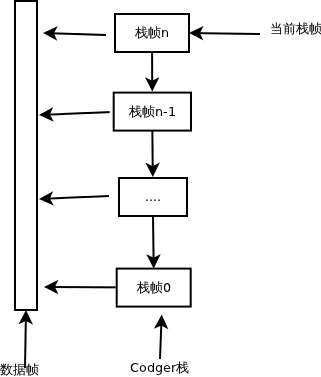
\includegraphics[scale=0.5]{EgThread.png}
\caption{线程对象的结构}
\label{fig:eg_thread}
\end{figure}

每当一个线程对象被创建时,它将会得到自己的pc寄存器,sp 寄存器,一个数据栈,以及一个Codger栈。寄存器pc的值总是会指向下一条执行的字节码;数据栈用于保存在计算过程中的临时对象和操作数;寄存器sp总是指向数据栈的栈顶;Codger栈总是存储Codger方法的调用状态,包括它被调用时传进来的参数值,它的返回值,局部变量等。

Codger方法指该方法在Codger源程序定义方法,如果一个方法调用是用c语言实现的,那么该方法被称为本地方法。Codger栈是由许多栈帧组成,一个栈帧包括一个Codger方法调用状态,当调用一个Codger方法时,会将一个新的帧栈压入到Codger栈中,当方法返回时,这个栈帧会作Codger栈中弹出并抛弃。
\subsection{模块对象}
模块是Codger组成源程序文件的一种基本的方式,模块也是一种的对象,模块对象可以赋值给一个变量,可以保存在集合对象中。每当一个源程序文件被加载时,虚拟机内部分生成一个模块对象来表示该文件,模块对象以一种等价的形式包含有源程序中的所有信息。模块对象(命名为A)可以import语句导入其它模块,在导入时,虚拟机首先检查被导入的模块是否被加载,如果已经加载,则直接返回给模块A;如果模块还没有被加载,意为着被导入的模块是每一次被其它模块导入,虚拟机会首先加载被导入的模块,然后再返回给模块A。

模块是一个可执行的对象,当模块第一次被加载时,模块对象中的字节码会被执行。在执行过程中所得到的对象可以通过export语句导出。当模块A导入模块B时,是把模块B存入到模块A当前作用域的一个变量里面,模块A可以访问成员的方法来得到模块B通过export导出的对象。

Codger的源程序被解析后会生成一个模块对象,在模块对象中保存了源程序中所有必要的信息,这些信息有:
\begin{enumerate}
\item 常量池:在程序中,布尔值,整数,浮点数,字符串,长整数,Nil这6种标量的数据类型是构成源程序的最基本的单位,它们不能在分解成其它更小的对象。在解析源文件完成时,源文件中出现的这6种标量数据类型都会被保存都常量池中。
\item 符号池:在源文件中出现的标识符,标识符指程序中出现在变量,函数名,类名等,它们都会被保存在符号池中。符号用于变量,成员访问或赋值,当源程序访问一个变量,虚拟机会在当前作用域中查找该变量的值,当前作用域可以被想象成一个符号表,里面存储了多个元素,每个元素由一个符号和一个值组成。当源程序访问对象成员时,虚拟机会从对象的符号表中查找值。虚拟机工作时,大部分时间都查询符号表或者时改变符号表中的值。
\item 带权限的符号池:对象的成员有访问权限,对象成员被其它对象访问时,虚拟机会检测是否有足够的访问权限,权限信息保存在带权限的符号中。当一个类对象创建一个实例对象时,实例对象的符号表中的符号使用的是带权限的符号。
\item 字节码池:在Codger源程序中,如果定义函数,或者是定义了类方法,解析器会它们单独生成字节码,这些字节码保存在字节码池中。函数对象创建时,会设置它在定义时所对应的字节码。
\item 模块字节码:解析器解析完成源文件后,源程序会转换成与之等价的这字节码,这些这节码被俣存在模块对象中。当模块第一次被加载时,这些字节码会被执行。
\item 符号表:模块的符号表保存模块export语句导出的对象。
\end{enumerate}
\subsection{数据栈}
数据栈在虚拟机运行过程中,负责保存运行时的临时对象,和指令所需要的操作数。Codger虚拟机除了寄存器sp,pc没有其它的寄存器,不使用多余的寄存器,一方面是保持虚拟机的简单性,另一方面是为了保证发生栈帧切换时,最小化栈帧上下文的数据保存与恢复。Codger中有许多的指令都需要操作数,这些需要操作数的指令运行时,它们的操作数来源于数据栈。例如代码a+b被转换成字节码后,有3个指令:
\begin{quote}
\begin{verbatim}
OP_LOAD_SYMBOL <a>
OP_LOAD_SYMBOL <b>
OP_PLUS
\end{verbatim}
\end{quote}
每一条指令是从当前作用域中查找变量a的值,并把值压入数据栈,每二条指令是从当前作用域中查找变量b的值,并把值压入数据栈。这时数据栈中已经有两个对象,执行到第三条指令OP\_PLUS时,它需要两个操作数,这两个操作数就会从数据栈中弹出,最后把运行的结果压入到数据栈中。
\subsection{栈帧}
栈帧由3部分组成:字节码,作用域,帧数据。
\begin{enumerate}
\item 字节码:保存了栈帧运行时的所有的指令,当一个Codger方法被调用时,栈帧会被创建,栈帧的字节码会被设置成Codger方法的字节码;或者是一个模块被第一次加载时,栈帧也会被创建,栈帧的字节码会被设置模块的字节码。
\item 作用域:用于保存运行时变量的值,每个作用域都有上层作用域,如果栈帧从Codger方法调用时创建,则作用域的上层作用域会被设置成Codger方法所在的作用域;如果栈帧是模块第一次加载时创建,则作用域的上层作用域会被设置成为空值。在栈帧执行的过程中,如是创建了函数对象,函数对象会对栈帧的作用域引用,保存在函数对象中,当栈帧退出时,栈帧的作用域并不会立即被销毁,只有在栈帧中创建的所有函数对象都销毁时,该作用域才会被销毁。Codger就是通过这种机制实现匿名函数。
\item 帧数据有:pc,sp值,返回值,属主对象。
\begin{enumerate}
\item pc,sp值用于在发生栈帧上下文切换时,保存和恢复栈帧运行时的信息;
\item 栈帧运行到返回指令时,会把返回值保存栈帧返回值里面。
\item 属主对象用于权限检测,假设现在的属主对象为A,执行到一条成员访问指令时,会从数据栈中取出操作数B,这时虚拟机会进行判断A与B是否为同一个对象,如果是,则表示对象A访问自身的成员;如果不是,则表示对象B的成员被对象A被访问。
\end{enumerate}
\end{enumerate}
\subsection{异常处理}
在程序运行的时候,可能会出现会多不同类型的异常,例如访问对象不存在的成员时,虚拟机会抛出NameErr类型的异常;访问数组对象中的元素时,下标越界,虚拟机会抛出IndexErr异常。这些异常可以使用异常捕获语句捕捉到。

当异常抛出时,虚拟会从Codger栈的顶部开始,依次遍历每一个栈帧,直到找到一个可以处理异常的栈帧为直。如果所有栈帧都不能处理抛出的异常,则虚拟机会把出错信息输出,并停止程序的运行。
\subsection{字节码}
Codger虚拟机在运行时,不停的执行当前栈帧的字节码,这是一个循环的过程,每次循环内容为:
\begin{enumerate}
\item 查测是否有异常产生,如果有则外理异常
\item 读入pc寄存器指向的指令,并更新pc值指向下一条运行的指令
\item 根据指令的类型,完成其相应的功能。
\end{enumerate}
